\documentclass{article}
\usepackage{amsmath}
\usepackage{todonotes}
\usepackage{color,soul}
\usepackage{caption}
\usepackage{subcaption}
% if you need to pass options to natbib, use, e.g.:
%     \PassOptionsToPackage{numbers, compress}{natbib}
% before loading neurips_2020

% ready for submission
%\usepackage{neurips_2020}

% to compile a preprint version, e.g., for submission to arXiv, add add the
% [preprint] option:
     \usepackage[preprint]{neurips_2020}

% to compile a camera-ready version, add the [final] option, e.g.:
%     \usepackage[final]{neurips_2020}

% to avoid loading the natbib package, add option nonatbib:
     \usepackage[nonatbib]{neurips_2020}

\usepackage[utf8]{inputenc} % allow utf-8 input
\usepackage[T1]{fontenc}    % use 8-bit T1 fonts
\usepackage{hyperref}       % hyperlinks
\usepackage{url}            % simple URL typesetting
\usepackage{booktabs}       % professional-quality tables
\usepackage{amsfonts}       % blackboard math symbols
\usepackage{nicefrac}       % compact symbols for 1/2, etc.
\usepackage{microtype}      % microtypography


\title{Exploring the Effects of Copy Number Alternations on Single Cell Embeddings in Cancer}
\author{Rebecca Boiarsky, Romain Lopez, Jan-Christian Hütter, Aviv Regev}
\date{August 5, 2023}

\begin{document}

\maketitle

\section{Introduction}

Elucidating elements of cancer biology that are common between different cancer types and subtypes is of great interest to the oncology community. Much progress has been made in identifying recurrent genetic drivers of tumor initiation and progression \citep{alexandrov2020repertoire}, but shared cellular phenotypes have been harder to pin down due to the vastly different transcriptional profiles between different tumor types. Moreover, even identifying cells with similar phenotypes among multiple patients with the same cancer type can be laborious owing to the widescale transcriptional differences between tumors from different patients. Dimensionality reduction and clustering are prototypical parts of single cell RNA-sequencing (scRNA-seq) analysis and are meant to elucidate groups of cells that share gene expression programs and allow for differential expression analysis between cell clusters\citep{wolf2018scanpy, butler2018integrating}. In cancer, this step of the workflow is often confounded by overwhelming differences between the transcriptional profiles of tumors from different patients, obscuring our ability to use standard pipeline tools such as principal component analysis (PCA) and t-stochastic neighbor embedding (tSNE) to embed cells in a latent space that relates information about cell state and disease status. Instead, cells often separate by patient, obscuring the ability to readily explore cell subtypes and gene expression activity across patients in the latent space \citep{fan2020single, tirosh2016dissecting, boiarsky2022single, gavish2023hallmarks}. As somatic copy number events are a common occurrence in tumor samples, we hypothesize that distinct copy number alternations (CNAs; used interchangeably with copy number variations, CNVs, throughout) across patients drive these large-scale transcriptional differences between tumors.

In this work, we investigate the effect of copy number variation on gene expression and explore approaches for correcting for copy number differences between tumors when embedding cells into a latent space. We aim to generate discussion about the role of CNAs in driving distinct transcriptional profiles between tumors, and the efficacy and pitfalls of different computational approaches for correcting for CNAs when embedding single cells in the context of cancer. %what drives patient tumors to be transcriptionally distinct, what features would be ideal   demonstrate how projecting tumor cells into a ``copy number free" latent space allows for recovery of shared cell subtypes from distinct patients.

\section{Related work}
\subsection{Effects of somatic CNA on gene expression}
While the prevalence and mechanisms of copy number events in cancer is well studied \citep{hastings2009mechanisms}, there has been limited prior work exploring the downstream effects of CNAs on gene expression \citep{shao2019copy, bhattacharya2020transcriptional}.

\subsection{Batch correction for single cell RNA-seq data}
Multiple methods exist for performing batch correction on single cell data in order to bring cells from disparate batches closer together in a latent space such as scVI \citep{lopez2018deep}, scPhere \citep{ding2021deep}, Harmony \citep{korsunsky2019fast}, and Seurat V3 \citep{stuart2019comprehensive}. 

\subsection{Identifying latents that are shared vs. unique between samples}
Instead of correcting for batch variables that drive certain cells apart, a different approach to finding share patterns of transcription between different groups of cells is to identify latent factors that are shared between the groups, even while other factors are not. LIGER \citep{welch2019single} and DIALOGUE \citep{jerby2022dialogue} are non-negative matrix factorization (NMF) based approaches to acheiving this, while multiGroupVI \citep{weinberger2022disentangling} and MrVI \citep{boyeau2022deep} are two autoencoder based approaches to solve this problem. In particular, MrVI learnes two separate latent spaces, one which is batch-variable "aware," and one that is batch-variable "unaware." This setup may be desirable in the cancer setting, as a hierarchical latent space may allow a practitioner to choose whether to view the "CNV-aware" latent space, as CNVs may correlate with aspects of important disease biology, or the "CNV-unaware" latent space, in which it may be easier to identify phenotypes present in subsets of cells from different tumors.

\section{Experiments and Results}
\subsection{Datasets}
We worked with three clinical single cell RNA-sequencing datasets from cancer:
\begin{itemize}
    \item The multiple myeloma (MM) dataset \citep{boiarsky2022single} contained 29,387 plasma (putative cancer cell of origin) and myeloma cells from 26 patients at varying disease stages and 9 healthy donors.
    \item The synovial sarcoma (SyS) dataset \citep{jerby2021opposing} contained 16,872  malignant, immune, and stromal cells from 12 human SyS tumors.
    \item The colorectal cancer (CrC) dataset \citep{lee2020lineage} contained 21,657 malignant, immune, and stromal cells from 15 human CrC tumors (Supplementary Note 1).
\end{itemize}

\subsection{Characterizing the effect of copy number on single cell gene expression}
\label{sec:CNA_res}

In order to estimate copy number profiles from single cell RNA-sequencing data, we ran inferCNV on the MM and SyS datasets, and used the results of inferCNA  provided by the authors of \cite{gavish2023hallmarks} for the CrC dataset. The output from these methods were gene level estimates of relative copy number change in each cell. 

We sought to understand the role of copy number in driving gene expression differences between tumors. Given the estimated CNV profiles of each cell, we interrogated whether genes unique to individual tumors were involved in copy number changes more often than they would be by chance. Taking the SyS dataset as an example, we calculated differentially expressed genes (DEGs) between the cells in a given tumor vs. all other tumors (Methods). Each tumor had between 491 and 7,224 DEGs, with a mean of 4,889 DEGs per tumor. Of the DEGs, on average 20.5\% were involved in a CNA (range [8.5, 40.3]). These numbers reveal that the majority of genes unique to a given tumor are not directly involved in a copy number event (Figure \ref{fig:lfc_cnv}). 
%\todo[]{mention whether this held true across the other datasets too}
%\todo[]{need a statistic here: calculate the probability of getting that number of CNV genes in the DEG set if all genes were equally likely (the null), and show it's less than 0.05?}

While it seemed that gene dosage change as a direct result of deletion or duplication does not account for most differential expression between tumors, we next investigated whether CNAs might still have a major influence on the unique gene profiles of each tumor through 1) exceptionally large fold changes for DEGs that were involved in CNAs compared to those that were not or 2) copy number events involving transcription factors driving differential expression of many downstream target genes. For 9 out of 12 tumors in the SyS dataset, the fold changes of DEGs involved in a CNA were not significantly more extreme than those of DEGs not involved in a CNA (Wilcoxon rank sum test). We downloaded a list of 795 transcription factors from the JASPAR database \citep{castro2022jaspar}, 617 of which overlapped with the gene names in the SyS dataset. For a given tumor, most of the genes affected by CNAs were not transcription factors \ref{fig:cnv_tf}. 
%\todo[]{these numbers seem low - is there a better database?}
%\todo[]{looking at their downstream targets}

\begin{figure}[h!]
     \centering
     \begin{subfigure}[b]{0.45\textwidth}
         \centering
         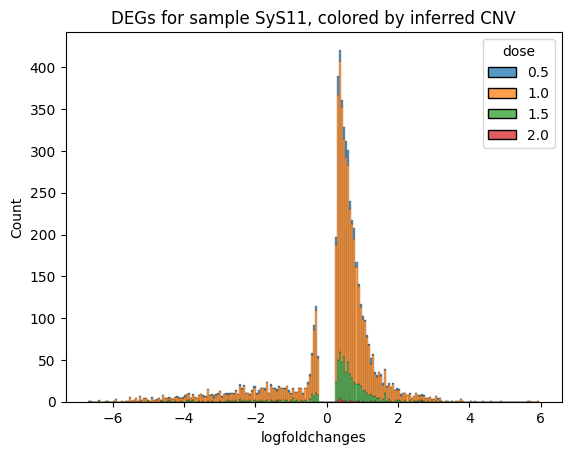
\includegraphics[width=\textwidth]{figures/sys11_deg_cnv_overlap.png}
         \caption{For representative sample Sys11, a histogram of the log fold changes for differentially expressed genes, with each DEG colored by its inferred CNA dosage.}
         \label{fig:lfc_cnv}
     \end{subfigure}
     \hfill
     \begin{subfigure}[b]{0.45\textwidth}
         \centering
         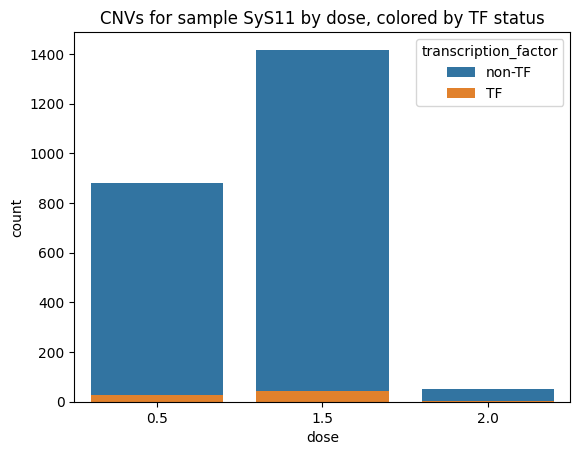
\includegraphics[width=\textwidth]{figures/sys11_cnv_tf_overlap.png}
         \caption{For representative sample SyS11, a histogram of the inferred dosage change for genes with copy number alterations, colored by whether or not the gene is listed as a transcription factor in the JASPAR database.}
         \label{fig:cnv_tf}
     \end{subfigure}
        \caption{Relationship between DEGs and CNVs in representative Synovial Sarcoma sample.}
        \label{fig:cnv_deg}
\end{figure}


\subsection{Generative model for copy number correction}
Given our results in section \ref{sec:CNA_res} which showed that the direct gene dosage effect of CNAs does not account for the majority of transcriptional differences between tumors, we explore correcting for CNAs in a non-linear fashion. We use the scvi-tools framework \citep{gayoso2022python}, which provides functionationality to correct for continuous covariates associated with each cell while embedding the cells to a latent space using a variational autoencoder. We compared the results of 3 different generative models, shown in Figure \ref{fig:gen_models}. We hypothesize that while embedding cells without any correction (Figure \ref{fig:vanilla_scvi}) clusters cells from different patients separately in the latent space, performing batch correction based on patient ID (PID) (Figure \ref{fig:scvi_pid}) may be too blunt a correction, obscuring meaningful biological differences between patients. We hypothesize that correcting for CNV profiles (Figure \ref{fig:scvi_cnv}) may overcome a significant portion of transcriptional differences between patients in a principled manner, such that a practitioner could know that the effects of CNAs should be minimized, but that other meaningful patient differences (eg. disease subtype) should still be captured in the latent space. To this end, we used principal component analysis (PCA) to reduce the dimensionality of each cell's CNA profile from $g$ genes to 20 dimensions, and then retained the top 5 principal components (PCs) that explained the most variance among CNA profiles, and input this vector as a per-cell batch variable.

\begin{figure}[h]
     \centering
     \begin{subfigure}[b]{0.3\textwidth}
         \centering
         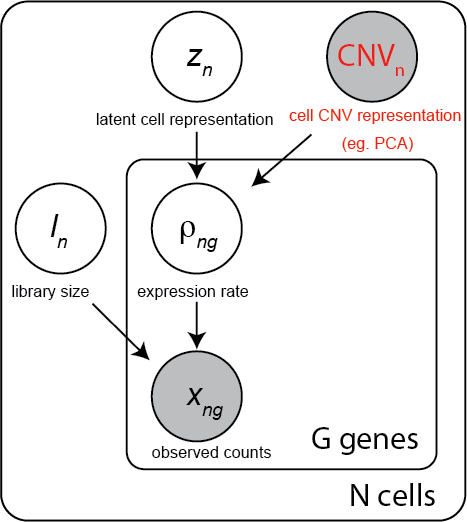
\includegraphics[width=\textwidth]{figures/scvi_cnv.png}
         \caption{A plate representation of the generative model used when correcting for CNA profiles as a continuous covariate.}
         \label{fig:scvi_cnv}
     \end{subfigure}
     \hfill
     \begin{subfigure}[b]{0.3\textwidth}
         \centering
         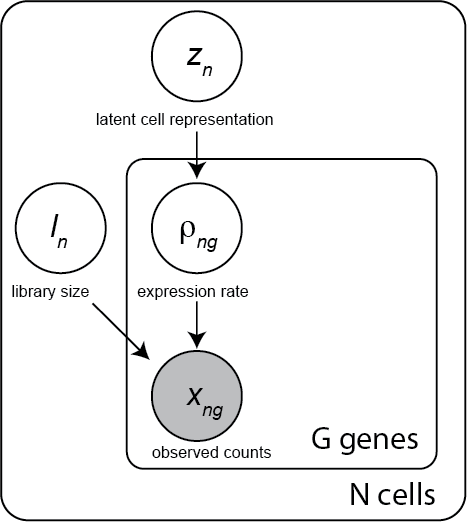
\includegraphics[width=\textwidth]{figures/vanilla_scvi.png}
         \caption{A plate representation of the generative model used for scVI without any batch correction.}
         \label{fig:vanilla_scvi}
     \end{subfigure}
          \hfill
     \begin{subfigure}[b]{0.3\textwidth}
         \centering
         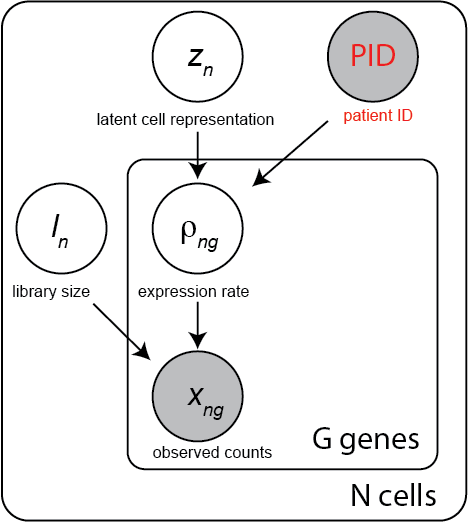
\includegraphics[width=\textwidth]{figures/scvi_pid.png}
         \caption{A plate representation of the generative model used when correcting for patient ID as a continuous covariate.}
         \label{fig:scvi_pid}
     \end{subfigure}
        \caption{In our main set of experiments, we compared the results of three generative models of gene expression, each represented above. Red text emphasizes the variable that was corrected for in a given model.}
        \label{fig:gen_models}
\end{figure}



\subsection{Evaluation setup}

In evaluating the effect of each correction scheme (no correction, correcting for PID, or correcting for CNV), we assessed the resulting latent representation of each cell using a few metrics:
\begin{enumerate}
    %\item The extent to which CNV was present in the latent space, quantified by the $R^2$ (coefficient of determination) for a linear regression model predicting a cell's CNV profile from its latent embedding. We expect this value to be lowest in the latent space which corrected for CNV.
    \item The extent to which PID was present in the latent space, quantified by the average accuracy for a logistic regression model predicting which patient a cell originated from given its latent embedding. We expect this value to be highest in the latent space with no batch correction, lowest in the latent space that corrected for PID, and intermediate in the latent space that corrected for CNV, since CNV profiles are patient-specific.
    \item The extent to which cells clustered according to meaningful biology in the latent space. For this metric, we used the 41 gene meta-programs (MPs) defined in recent work that studied transcriptional heterogeneity across 1,000 tumors \citep{gavish2023hallmarks}, and assessed how spatially autocorrelated each MP was in the latent space using Geary's C value, which has previously been applied to assess single cell similarity (see Methods) \citep{geary1954contiguity, detomaso2019functional}. Briefly, Geary's C is calculated as $$C=\frac{(N-1)\sum _{i}\sum _{j}{w}_{ij}{({x}_{i}-{x}_{j})}^{2}}{2W\sum _{i}{({x}_{i}-\overline{x})}^{2}}$$ where $N$ denotes the total number of cells, $w_{ij}$ refers to the connectivity weight between cells $i$ and $j$ in a KNN neighborhood graph, $x$ represents a value of interest, in our case the level of gene MP activity, $W$ is the sum of all weights, and $\overline{x}$ is the mean of $x$. Following \cite{detomaso2019functional}, we report $C^* = 1-C$, such that scores generally range between 0 and 1, with 0 representing no correlation, and 1 representing high correlation.   
\end{enumerate}

\subsection{Experimental results}

We ran the three scVI models described in Figure \ref{fig:gen_models} each five times, in order to capture the variation in latent space resulting from the stochasticity of the model and learning procedure. We found that results were qualitatively similar across the five runs for each model. In Figure \ref{fig:umaps_clinical}, we share unified manifold approximation and projection (UMAP) plots representing the latent space learned using each model for the multiple myeloma dataset, coloring cells by patient ID and disease stage in order to aid in tracking their relative positions under the three different models. We then evaluated each latent space according to the metrics described above.

\begin{figure}[h]
     \centering
     \begin{subfigure}[b]{\textwidth}
         \centering
         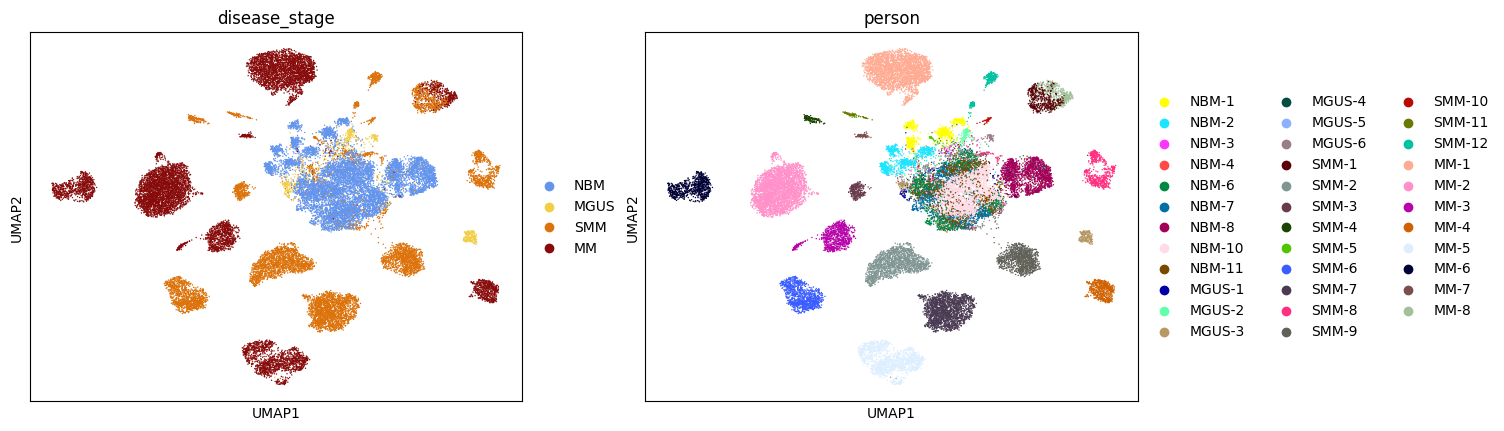
\includegraphics[width=\textwidth]{figures/umap_scvi_seed1_clinicalcovars2.png}
         \caption{UMAP of cells in latent space after running scVI with no correction.}
         \label{fig:vanillascvi_umap}
     \end{subfigure}
     \hfill
     \begin{subfigure}[b]{\textwidth}
         \centering
         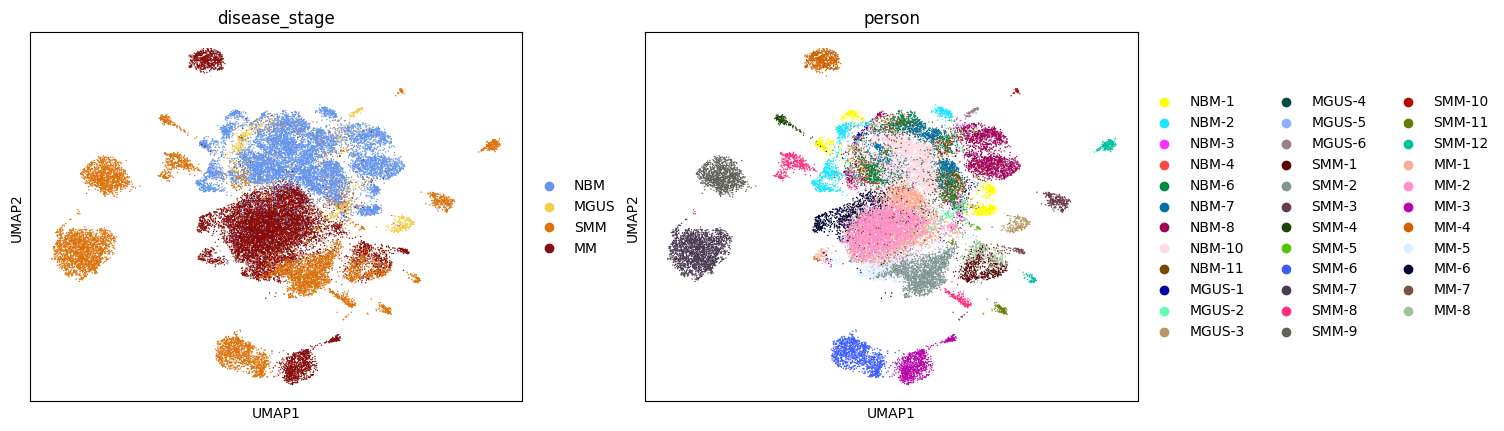
\includegraphics[width=\textwidth]{figures/umap_scvi_CNVcont_seed1_clinicalcovars2.png}
         \caption{UMAP of cells in latent space after running scVI and correcting for CNAs, using the first seven principal components.}
         \label{fig:cnv_umap}
     \end{subfigure}
          \hfill
     \begin{subfigure}[b]{\textwidth}
         \centering
         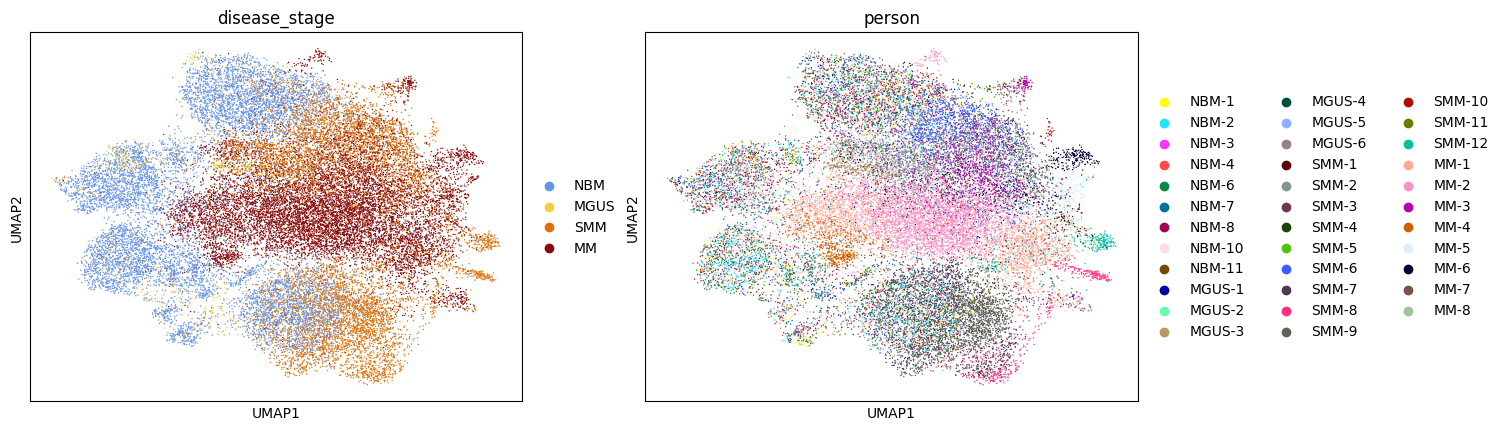
\includegraphics[width=\textwidth]{figures/umap_scvi_batchperson_seed1_clinicalcovars2.png}
         \caption{UMAP of cells in latent space after running scVI and correcting for patient ID.}
         \label{fig:pid_umap}
     \end{subfigure}
        \caption{UMAP plots of the latent space learned using three different correction schemes for the multiple myeloma dataset. Cells are colored by disease stage (left; NBM=normal bone marrow, MGUS=monoclonal gammopathy of undetermined significance, SMM=smoldering multiple myeloma, MM=myeloma) and patient ID (right).}
        \label{fig:umaps_clinical}
\end{figure}

%\subsubsection{Presence of CNV in the latent space.}


\subsubsection{Presence of PID in the latent space.}
As expected, across all datasets, PID is least predictable from the model which explicitly regresses out the PID. Further, the fact that PID is still predictable from the latent spaces corrected for CNV reflects that while CNV profiles are correlated with PID, they contain only a subset of patient-specific information. We note that as we increase the number of CNV PCs that we use in the correction, the accuracy of predicting PIDs from the CNV-corrected latent space further decreases, reflecting the fact that the CNV principal components may in fact be capturing patient information, but that the granularity of the correction can be tuned by choosing how many PCs to include in the correction.

\subsubsection{Spatial autocorrelation of gene MPs in the latent space.}
In Figure \ref{fig:gearys_mm_results}, we present results for the spatial autocorrelation of some representative MPs in the MM dataset across the three different latent space learned (each latent space was run with five different seeds to capture stochasticity; for full results, see Supplementary Figures). We chose to present the six MPs that had the highest mean $C^*$ value in the uncorrected latent space, as these are gene programs with high activity in the MM dataset. We find that while the spatial autocorrelation structure is lost when correcting for PID, it is retained in the latents that instead corrected for CNVs.

\begin{figure}
    \centering
    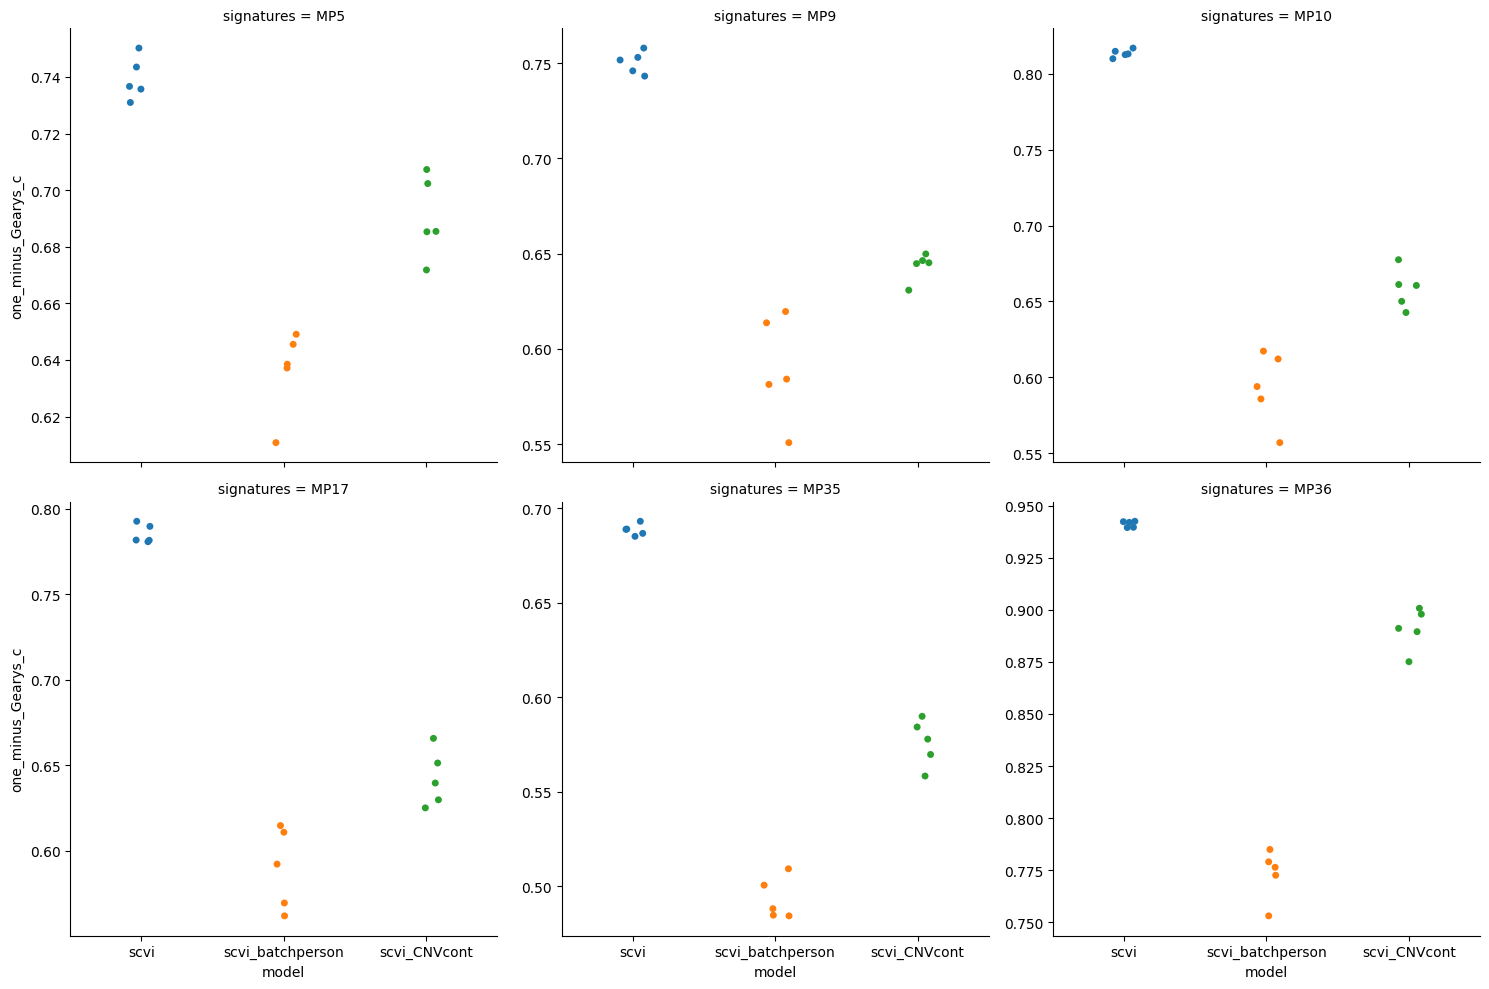
\includegraphics[width=\textwidth]{figures/gearys_c_mm_top6.png}
    \caption{For the MM dataset, $C^*$ (1-Geary's C) for the six gene meta-programs (MPs) with the highest mean activity in the uncorrected latent space (mean taken across 5 runs of scVI). We find that while the spatial autocorrelation structure is lost when correcting for PID, it is retained in the latents that instead corrected for CNVs}
    \label{fig:gearys_mm_results}
\end{figure}

\section{Discussion}
While it is believed that CNAs play a large part in driving the wide-scale transcriptional differences between tumors from different patients, there is limited research characterizing the extent of their influence on transcription relative to other factors that can affect transcription, such as point mutations, cytogenetic changes, and influences from the microenvironment. Additionally, the effect of CNAs on transcription may vary between different cancer types or subtypes. There have been some reports of correlation between disease biology and CNAs, and therefore it is possible that by regressing out CNAs from a latent cell representation, one will also regress out important aspects of disease biology. For example, \cite{gavish2023hallmarks} report multiple correlations between specific CNAs and expression of specific gene meta-programs, and these associations vary between different cancer types. In medulloblastoma, \cite{gold2022developmental} report correlations between specific CNAs and cell proliferation as well as the developmental stage of the malignant cells, respectively. An undesirable effect of regressing out CNAs may be regressing out important cellular phenotypes, such as these, and we therefore advise caution in implementing this kind of approach.

In the form we presented here, correcting for CNVs represents an intermediate correction between no correction at all, and correcting for each patient individually. Our exploration of CNV correction was motivated by the idea that the CNV profiles will be able \textit{group} patients in a meaningful way, thus retaining some inter-patient structure in the learned latent space. In practice, with the small amount of data used here, it is not clear that the patient groupings are biologically meaningful, and future work is needed to understand how CNVs vary between patients and how this variation can be used to group patients together before doing a batch correction.

\clearpage
\bibliographystyle{unsrtnat}
\bibliography{references}
\clearpage
\section{Supplementary Info}

\textbf{Supplementary Note 1.} We used the version of the \cite{lee2020lineage} CrC dataset that was preprocessed by \cite{gavish2023hallmarks} and available on the Curated Cancer Cell Atlas (3CA; \url{https://weizmann.ac.il/sites/3CA}). As Gavish et al. note, this dataset contains 15 colorectal carcinoma samples from the SMC cohort, sequenced at the Samsung Medical Center in Seoul. The full cohort consists of 23 tumor samples – 8 were excluded due to insufficient CNA signal. Cells with fewer than 1000 genes detected were also excluded.

\section{Extended Methods}

\subsection{Calculation of DEGs}
To calculate differentially expressed genes (DEGs) between different tumors, we used a Wilcoxon rank sum test to compare the log-normalized gene expression in different tumors. Any gene with a Benjamini-Hochberg adjusted p-value $<0.1$ was retained as a DEG. Fold changes were calculated as the ratio of log-normalized expression + offset for cells in a given tumor, to that of cells in other tumors. The offset used is half of the non-zero minimum of log-normalized gene expression in the dataset. For datasets that contained non-malignant cells (eg. the CrC and Sys datasets), we had an additional post-processing step where we calculated patient-specific DEGs for all other annotated cell types (eg. T cells from patient A vs. T cells not from patient A), and removed these non-malignant patient specific genes from our list of malignant DEGs, such that the malignant DEGs reflect differences that arise specifically between tumors, not simply between patients. For example, we saw the sex gene \textit{XIST} removed from the tumor DEG list after post-processing in this way.

\subsection{The scVI generative model}
Given scRNA-seq counts $x_{ng}$ and copy number information $c_{ng}$ for each gene $g$ in each cell $n$ (which can be estimated from the RNA-seq data itself using software like InferCNV), we propose a generative model of single cell gene expression of the following form (corresponding to Figure \ref{fig:scvi_cnv}):\\

\begin{align}%{ll} 
{z_n} & {\sim {\mathrm{Normal}}\left( {0,I} \right)} \\ 
{\ell _n} & {\sim {\mathrm{log}}\,{\mathrm{normal}}\left( {\ell _\mu ,\ell _\sigma ^2} \right)} \\ 
{\rho _n} & { = f_w\left( {z_n,c_{ng}} \right)} \\ 
{w_{ng}} & {\sim {\mathrm{Gamma}}\left( {\rho _n^g,\theta } \right)} \\ 
{x_{ng}} & {\sim {\mathrm{Poisson}}\left( {\ell _nw_{ng}} \right)}
\end{align}

where $l_n$ represents the library size (or total counts) in each cell, $f_w$ is a function parameterized by a neural network, and $\theta \in {\Bbb R}_ + ^G$ denotes a gene-specific inverse dispersion, estimated via variational Bayesian inference.

\subsection{Running scVI}
Prior to running scVI, each dataset was limited to 5,000 highly variable genes (HVGs), in order to speed up training times in scVI. HVGs were chosen using the function \texttt{scanpy.pp.highly\_variable\_genes()} with the argument \texttt{flavor="seurat\_v3"}. scVI was run as implemented in the scvi-tools package version 1.0.0. To correct for CNV, we called the \texttt{scvi.model.SCVI.setup\_anndata} function with the argument \texttt{continuous\_covariate\_keys} set to the PCA-based CNV features in the anndata .obs matrix, and to correct for PID, we called the same function with the argument \texttt{batch\_key} set to the column in the anndata .obs matrix containing patient identifiers. We opted to model the likelihood of gene expression counts using the negative binomial distribution, as implemented in scvi-tools.


%\subsection{Calculation of MP score}

%\subsection{Calculation of Geary's C}

\section{Code Availability}
inferCNV is available at \url{https://github.com/broadinstitute/infercnv}. inferCNA is available at \url{https://github.com/jlaffy/infercna}. %Analysis scripts for results in this paper are available at \hl{[insert name of repo once cleared by legal]}.





\end{document}

Random notes:
    -  UMAP plots may not be an ideal way to see our learned embeddings $z$, since they mostly preserve local distances, and cells from the same patient will likely still be more similar to each other even after correcting for CNVs. Hierarchical clustering may be a better choice? Other options?
    -  For cancers with known subtypes, we would expect to see cells cluster by subtype rather than by patient (eg. in MM there are subtypes characterized by different translocation events which exhibit distinct transcriptional patterns)
    - might be a good idea to do hierarchical clustering of cells and see how things cluster, just as a very different method from scvi

